\documentclass[12pt]{article}
\usepackage[utf8]{inputenc}
\usepackage{float}
\usepackage{amsmath}

\usepackage[hmargin=3cm,vmargin=6.0cm]{geometry}
\topmargin=-2cm
\addtolength{\textheight}{6.5cm}
\addtolength{\textwidth}{2.0cm}
\setlength{\oddsidemargin}{0.0cm}
\setlength{\evensidemargin}{0.0cm}

\usepackage{indentfirst}
\usepackage{amsfonts}
\usepackage{graphicx}
\usepackage{listings}
\usepackage{xcolor}

\definecolor{codegreen}{rgb}{0,0.6,0}
\definecolor{codegray}{rgb}{0.5,0.5,0.5}
\definecolor{codepurple}{rgb}{0.58,0,0.82}
\definecolor{backcolour}{rgb}{0.95,0.95,0.92}

\lstdefinestyle{mystyle}{
  backgroundcolor=\color{backcolour},
  commentstyle=\color{codegreen},
  keywordstyle=\color{magenta},
  numberstyle=\tiny\color{codegray},
  stringstyle=\color{codepurple},
  basicstyle=\ttfamily\footnotesize,
  breakatwhitespace=false,
  breaklines=true,
  captionpos=b,
  keepspaces=true,
  numbers=none,
  numbersep=5pt,
  showspaces=false,
  showstringspaces=false,
  showtabs=false,
  tabsize=2
}

\lstset{style=myStyle}

\begin{document}

\section*{Student Information }
%Write your full name and id number between the colon and newline
%Put one empty space character after colon and before newline
Full Name : Murat Bolu \\
ID Number : 2521300 \\

% Write your answers below the section tags
\section*{Answer}

\subsection*{a)}
\noindent
The Octave code is as follows,
\begin{lstlisting}[language=Octave]
% Load statistics module for inverse standard normal distribution
pkg load statistics;

% Define the constants
poissLambdaBulk = 50;
poissLambdaContainer = 40;
poissLambdaOil = 25;

alphaBulk = 60;
alphaContainer = 100;
alphaOil = 120;

gamLambdaBulk = 0.1;
gamLambdaContainer = 0.05;
gamLambdaOil = 0.02;

weightThreshold = 300000;

alphaProbability = 1 - 0.98;
epsilonDifference = 0.03;
% Calculate Monte Carlo study size
z_alpha = norminv(1 - alphaProbability/2);
sizeMonteCarlo = ceil(0.25 * (z_alpha/epsilonDifference)^2);

% Function to generate poisson and gamma random variables and calculate total cargo
function result = generateTotalSize(poissLambda, alpha, gamLambda)
  U = rand;
  i = 0;
  F = exp(-poissLambda);
  while (F < U);
    F += exp(-poissLambda) * poissLambda^i / gamma(i+1);
    i += 1;
  endwhile
  result = 0;
  for j = 1:i;
    result += sum(-1/gamLambda * log(rand(alpha, 1)));
  endfor
endfunction
% Number of times total cargo exceeded threshold
cargoExceeds = 0;
% Vector of total cargo sizes
sums = [];

for i = 1:sizeMonteCarlo;
  sumBulk = generateTotalSize(poissLambdaBulk, alphaBulk, gamLambdaBulk);
  sumContainer = generateTotalSize(poissLambdaContainer, alphaContainer, gamLambdaContainer);
  sumOil = generateTotalSize(poissLambdaOil, alphaOil, gamLambdaOil);
  sumAll = sumBulk + sumContainer + sumOil;
  sums = [sums, sumAll]; % Append to sums vector
  cargoExceeds += (sumAll > weightThreshold);
endfor

% Probability that the total cargo exceeded the threshold
probabilityExceeds = cargoExceeds/sizeMonteCarlo;
% X is average daily total cargo
X = mean(sums);
% Standard deviation of X
stdDevX = std(sums);

fprintf("Estimated probability: %.3f\nExpected weight: %.2f\nStandard deviation: %.2f\n", probabilityExceeds, X, stdDevX);
\end{lstlisting}

\noindent
with a screenshot of some outputs,

\begin{center}
  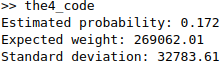
\includegraphics[scale = 1]{the4_output.png}
\end{center}

In this part, we calculated the size of the Monte Carlo study by using the $N
\geq 0.25(\frac{z_{\alpha/2}}{\varepsilon})^2$ formula. We did not have an
estimate for the probability $p$, so we used the highest possible value of
$p\cdot(1-p)$ which is $0.25$. We have the size of the Monte Carlo study as
$1504$. Then, for each type of ship, we generate the Poisson random variable to
determine the number of ships arriving. For each ship, we generate the
gamma-distributed random variable to determine its cargo weight. We calculate
the sum for each type of ship, then we calculate the total amount of cargo
weight in a day by summing three different type of ships. Then, we determine if
the total cargo weight passes the threshold. We repeat this process for $1504$
times, the size of our Monte Carlo study. Our estimated probability of a day
exceeding the cargo weight threshold is around $17\%$.

\subsection*{b)}

Our estimate for the average amount of total cargo weight that arrives to the
port every day is around $270$ thousand tons. We calculated this value by taking
the average of total cargo weight of every iteration.

\subsection*{c)}

Our estimate for the standard deviation of the average total cargo weight is
around $32$ thousand tons. We calculated this value by taking the standard
deviation of the sample generated by Monte Carlo simulation.

\end{document}
